% \definecolor{MidnightBlue}{cmyk}{0.98,0.13,0,0.43} % PANTONE 302
\pagecolor{yellow}
\color{black}

\bigskip

\begin{center}
{\Huge Recommender Systems}

{\LARGE Norm Matloff 

\medskip

University of California, Davis}

\bigskip

\vspace{0.5in}

% {\LARGE GPU, Multicore, Clusters and More}

\vspace{1in}

% \begin{figure}[ht]
% \color{white}
%    \begin{minipage}[b]{0.35\linewidth}
%       \includegraphics[width=1.2in]{Images/CUDALogo.jpg}
%    \end{minipage}
%    \hspace{2.5in}
%    \begin{minipage}[b]{0.35\linewidth}
%       \includegraphics[width=1.2in]{Images/OpenMPLogo.jpg}
%    \end{minipage}
% \end{figure}
%    \begin{minipage}[b]{0.35\linewidth}
%       \includegraphics[width=1.2in]{Images/MPILogo.jpg}
%    \end{minipage}

   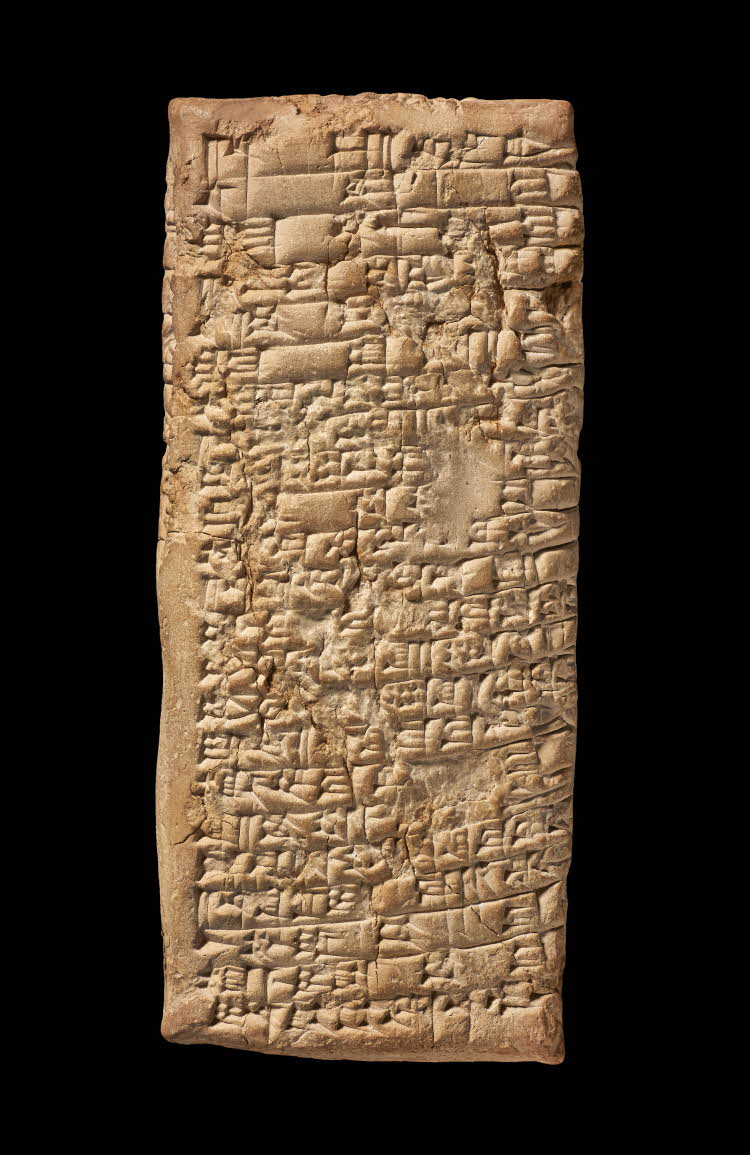
\includegraphics[width=1.2in]{Images/AncientYelp.jpg}

\end{center}

\vspace{1.5in}

See Creative Commons license at 
{http://heather.cs.ucdavis.edu/~matloff/probstatbook.html} 

This book is often revised and updated, latest edition available at
{http://heather.cs.ucdavis.edu/~matloff/158/PLN/ParProcBook.pdf} 

CUDA and NVIDIA are registered trademarks.


The author has striven to minimize the number of errors, but no
guarantee is made as to accuracy of the contents of this book.


\newpage

% \title{Programming on Parallel Machines} 
% 
% \author{Norman Matloff\\
%  University of California, Davis
%  \thanks{
%     { \bf Licensing:}
%     This work is licensed under a Creative Commons Attribution-No Derivative
%     Works 3.0 United States License. Copyright is retained by N. Matloff in
%     all non-U.S. jurisdictions, but permission to use these materials in
%     teaching is still granted, provided the authorship and licensing
%     information here is displayed in each unit. I would appreciate being
%     notified if you use this book for teaching, just so that I know the
%     materials are being put to use, but this is not required.}
% }
% 
% \date{}   
% 
% 
% \maketitle

